\chapter{Anwenderdokumentation}
\section{Produktzweck}
Eines der wohl wichtigsten Werkzeugen nicht nur im Studium, sondern 
auch in Berufen speziell in der Forschung und Entwicklung, sind B"ucher. 
Allerdings ist der Umfang von Fachliteratur nicht unbedingt klein und 
"uberschaubar. Au"serdem kann ein Fehlkauf sehr schnell ins Geld gehen, 
bei B"ucherpreisen von 50 EUR und mehr.\\
Wie w"are es also mit einem Werkzeug um Informationen "uber diese 
Werkzeuge "ubersichtlich bereit zu stellen.\\
Informationen wie Titel, Autor und ISBN werden von 
Migliedern verfasst und in einer Datenbank abgelegt. Aber 
damit nicht genug, es ist jedem Mitglied auch m"oglich Kommentare zu 
verfassen, z. B. wie ihm das Buch gefallen hat oder ob es bei Recherchen "uber gewisse Themen
hilfreich war oder nicht.\\
Um einen universellen Zugriff auf die Datenbest"ande der Literaturverwaltung zu gew"ahrleisten, 
erfolgt der Zugriff "uber dynamisch erzeugte HTML-Seiten, die einfach 
mit jedem Web-Browser "uber die Web-Adresse aufgerufen werden k"onnen.\\
Ein weiterer Vorteil, den dynamisch erzeugte HTML-Seiten bieten ist die freie Plattformwahl durch den Nutzer.

\section{Basismaschine und Ressourcenanforderungen}
Die Literaturverwaltung wird von einem Administrator auf einem Web-Server installiert und konfiguriert. Dies erm"oglicht jedem Nutzer einen ortsunab"angigen Zugriff auf die Datenbest"ande.\\
Es wird lediglich ein Web-Browser wie z. B. Firefox, Opera oder der Internet Explorer ben"otigt.\\
Die Anforderungen an die Hardware richten sich nach den Anforderungen des benutzten Web-Browsers.

\section{Nutzerklassen}
Es gibt drei Nutzerklassen:
\begin{enumerate}
\item Nutzer:\\
Nutzer ist jeder, der sich "uber einen Web-Browser auf die Seite begibt um Informationen abzurufen.\\
Der Nutzer besitzt keinerlei M"oglichkeiten Datenbest"ande anzulegen, zu ver"andern oder zu l"oschen. Er besitzt lediglich Lesezugriff auf die Literaturinformationen und Kommentare. \\

\item Mitglied:\\
Das Mitglied ist ein registrierte Nutzer, der sich durch sein Anmelden "uber die grafische Oberfl"ache mit einem LogIn-Namen und einem Passwort als solcher authentifiziert.\\
Als Mitglied darf man zus"atzlich zu den Rechten eines Nutzers neue Literatur anlegen oder bereits bestehende Titel bearbeiten und l"oschen.\\
Desweiteren besitzt jedes Mitglied das Recht, Kommentare zu verfassen sowie eigens erstellte Kommentare zu bearbeiten und zu l"oschen.\\
Was die Mitgliedsdaten betrifft, so darf jedes Mitglied die eigenen Nutzerdaten bearbeiten. Was die Rechte betrifft, so ist eine "Anderung ausschlie"slich durch einen Administrator m"oglich.\\

\item Administrator:\\
Zun"achst wird durch einen Administrator die Literaturverwaltung auf einem Web-Server installiert und konfiguriert.\\
Weiterhin ist der Administrator f"ur die Datenverwaltung und inbesondere f"ur die Mitgliedsverwaltung zust"andig, also z. B. f"ur die Pflege der Mitgliedsdaten.\\
Was die Rechte eines Administrators betrifft so sind diese allein auf Grund seines Aufgabengebietes unbeschr"ankt, d.h. er kann alle Daten sehen, erstellen, bearbeiten und l"oschen.\\ 

\end{enumerate}
\section{Bedienungsanleitung}
\subsection{Start der Anwenung}
Um den Literaturmanager zu starten muss man einen Web-Browser (hier Firefox 1.5.0.4) starten und die passende Internet-Adresse in das URL-Feld eintragen. Die URL kann man beim Administrator erfragen, da er den Web-Server zuvor konfiguriert.
\subsection{Die Hauptseite}
Hat man die richtige Web-Adresse eingegeben, so l"adt der Browser folgende Seite:\\
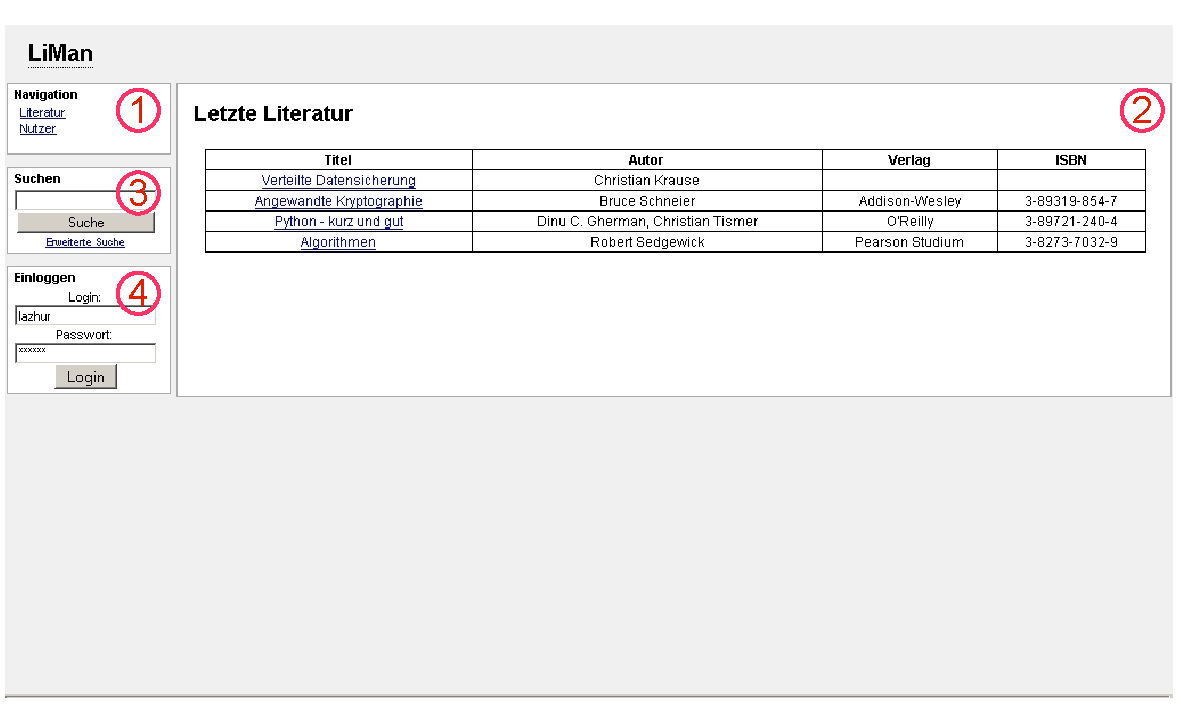
\includegraphics[scale=0.8]{screen1}\\
Die Hauptseite ist in vier Segmente aufgeteilt:\\
\begin{enumerate}
\item Navigation:\\
In dem Segment Navigation kann man nun zwischen zwei Men"upunkten w"ahlen:\\
Literatur und Nutzer\\
Auf diese beiden Punkte wird sp"ater genauer eingegangen.
\item Letzte Literatur:\\
Dieses Segment erm"oglicht einen "Uberblick der zuletzt get"atigten Literatureintr"age.
\item Suchen:\\
Die Suchfunktion erm"oglicht eine schnelle Recherche in den vorhandenen Literaturdaten. Die genauere Bedienung wird noch erl"autert.
\item Einloggen:\\
Hier kann sich jedes Mitglied mit seinem Login, also einem Namen und seinem Passwort bei dem Literaturmanager anmelden.\\
Sollte man keinen Login-Name und kein Passwort besitzen so muss man sich bei einem Administrator anmelden.\\
Auch wenn man sein Passwort vergessen hat, muss man einen Administrator kontaktieren.\\
\end{enumerate}
\subsection{Wie logge ich mich ein?}
Im Segment Einloggen auf der Hauptseite existieren zwei Editfelder, Login und Passwort.\\
Man gibt also in das obere Feld seinen Login-Namen und in das zweite Feld sein Passwort ein. Anschlie"send bet"atigt man den Button "Login" (1).\\
In der folgenden Abbildung ist der Abschnitt Einloggen einmal vergr"o"sert dargestellt.
Wir Loggen uns mit dem Namen 'Lazhur' und dem Passwort 'tescht' ein:\\
\begin{center}
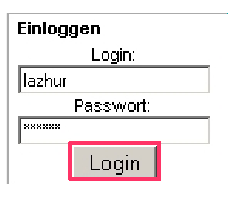
\includegraphics[scale=1.0]{login}\\
\end{center}
War die Anmeldung erfolgreich so erscheint folgende Anzeige und man ist als Mitglied eingeloggt:\\
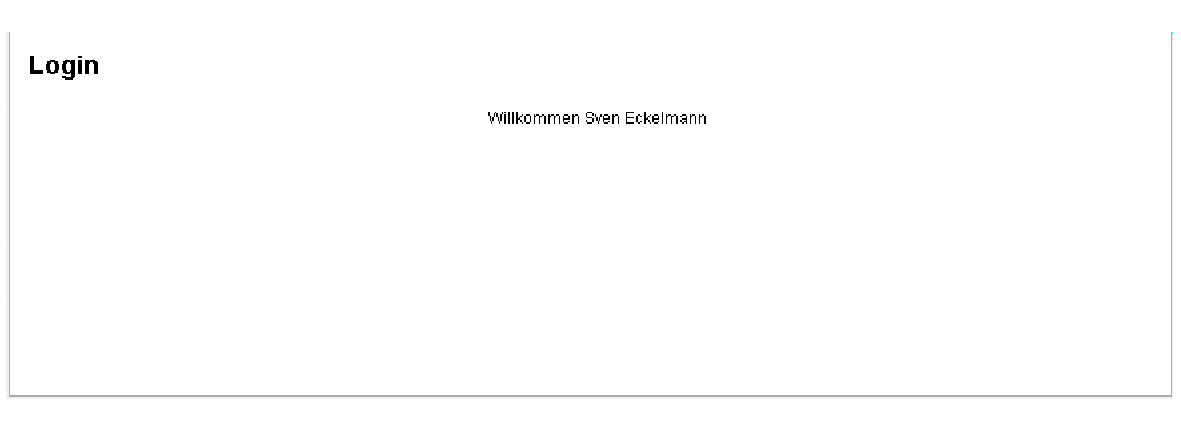
\includegraphics[scale=0.8]{login1}\\

\subsection{Wie finde ich eine Literatur?}
Um Informationen zu einem Literaturtitel zu erhalten bietet es sich an die Suchfunktion des Literaturmanagers zu nutzen. Hierzu kommen wir kurz auf das Bild des Hauptbildschirm weiter oben zur"uck:\\
Folgendes Bild verg"o"sert das Suchsegment (3):\\
\begin{center}
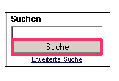
\includegraphics[scale=2.0]{suche}\\
\end{center}
Das Prinzip ist ganz einfach. Man gibt ein Stichwort zu einem Literaturtitel ein, z. B. ein Wort aus dem Titel oder den Namen des Autors, und dr"uckt den Suche-Button (1).\\
Gibt man z. B. den Begriff 'Python' ein so erscheinen alle Literaturtitel mit diesem Begriff. Die n"achste Abbildung zeigt einmal eine solche Trefferliste:\\
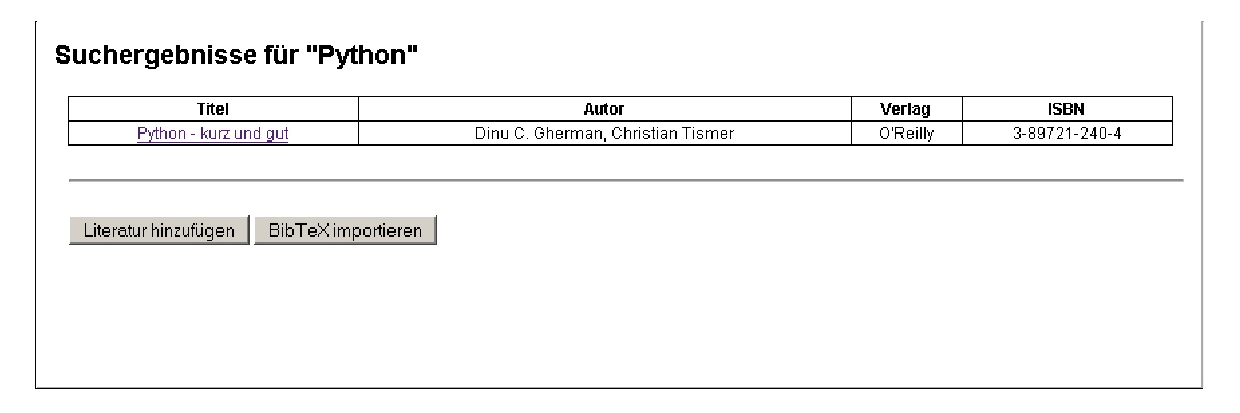
\includegraphics[scale=0.8]{treffer}\\
\subsection{Wie kann ich eine neue Literatur anlegen?}
Kommen wir nun vom Recherchieren zum bearbeiten und Pflegen der Literaturverwaltung.\\
Angenommen eine Literatur ist nicht in der Literaturverwaltung vorhanden und ein Mitglied m"ochte es darin aufnehmen.\\
Hierzu klicken wir zun"achst im Segment 'Navigation' auf den Punkt 'Literatur', daraufhin erscheint folgendes Fenster:\\
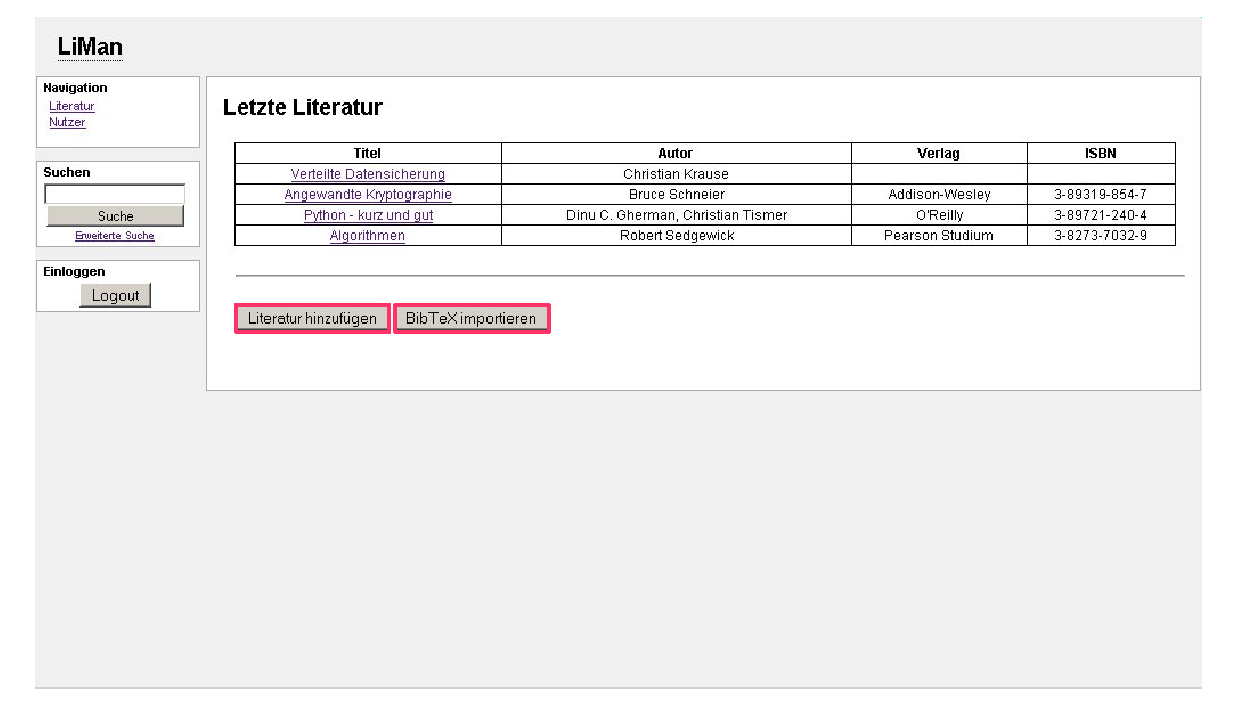
\includegraphics[scale=0.8]{lit_ins}\\
Dominiert wird das Segment von der Tabelle mit den Literatureintr"agen darunter befinden sich zwei Buttons, die nur dann erscheinen, wenn man sich als Mitglied angemeldet hat.\\
Der Button 'Literatur hinzuf"ugen' spricht wohl f"ur sich. Er erm"oglicht das hinzuf"ugen eines neuen Literaturtitels.\\
Der Button 'BibTex importieren' erm"oglicht es bereits vorgefertigte Literaturbeschreibungen im BibTex-Format zu importieren.\\
Klickt man nun auf den Button 'Literatur hinzuf"ugen' erscheint folgendes Formular:\\
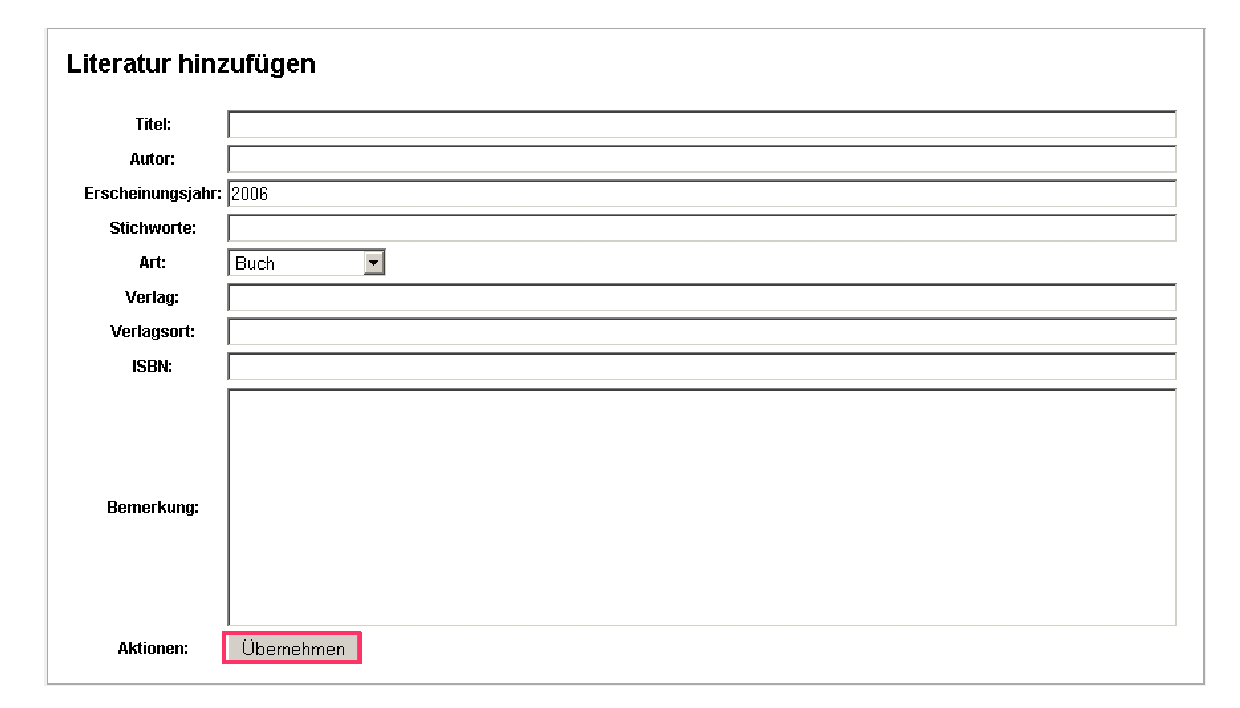
\includegraphics[scale=0.8]{lit_ins1}\\